\documentclass[11pt]{article}
\usepackage{amsmath, amssymb, amsthm}
\usepackage[margin=1in]{geometry}
\usepackage{float}
\usepackage{graphicx}
\usepackage{subcaption}
\usepackage{booktabs}
\usepackage{hyperref}
\usepackage[capitalise]{cleveref}
\usepackage{tikz}
\usetikzlibrary{shapes.geometric, arrows.meta, positioning, calc}

% Let two figure floats share a page instead of each claiming one.
\renewcommand{\topfraction}{0.92}
\renewcommand{\bottomfraction}{0.7}
\renewcommand{\textfraction}{0.07}
\renewcommand{\floatpagefraction}{0.8}
\setlength{\floatsep}{10pt plus 2pt minus 2pt}
\setlength{\textfloatsep}{12pt plus 2pt minus 3pt}

\newtheorem{theorem}{Theorem}
\newtheorem{lemma}{Lemma}
\newtheorem{assumption}{Assumption}
\newtheorem{remark}{Remark}

\begin{document}

\section{The Distance Route: Single-Stage Spectral Recovery}

This section establishes the exact recovery of tree splits using the sign pattern of the leading eigenvector of the double-centered distance matrix. Rather than relying on multi-stage refinement algorithms or demanding full knowledge of the eigenvector's shape, we pursue a purely spectral approach. By importing the structural Schur complement theory of Stone and Griffing \cite{stone2009fiedler} and the leave-one-out entrywise perturbation framework of Abbe et al. \cite{abbe2020entrywise}, the recovery guarantee emerges organically from the native geometry of the distance matrix.

\subsection{Population Geometry and the Spectral Target}
\label{sec:target}

Let $T$ be a weighted tree with $m$ leaves, and let $\mathcal{D}$ be the additive path-distance matrix between the leaves. We apply double centering with the orthogonal projector $H = I - \frac{1}{m}\mathbf{1}\mathbf{1}^\top$ to form the distance operator:
\begin{equation}
\mathcal{B} := H \mathcal{D} H
\end{equation}
The recovery algorithm classifies leaves by the sign pattern of $u^{(1)}$, the unit eigenvector of $\mathcal{B}$ belonging to its largest-magnitude eigenvalue.

Griffing \cite{griffing2012} showed that $-\frac{1}{2}\mathcal{B}$ is exactly the Moore-Penrose pseudoinverse of the tree Laplacian Schur-complemented onto the leaves. Consequently, $u^{(1)}$ is mathematically identical to the Fiedler vector of this Schur complement. By the structural theorems of Stone and Griffing \cite{stone2009fiedler}, this vector unconditionally partitions the leaves into a valid split of the tree.

\begin{lemma}[Target Geometry \cite{stone2009fiedler}]
The sign pattern of $u^{(1)}$ corresponds to a bipartition of the leaves cut by a single edge in $T$. Furthermore, $u^{(1)}$ has no zero coordinate, yielding a strictly positive margin $\delta_* := \min_i |u_i^{(1)}| > 0$.
\end{lemma}

Because we do not assume the tree is perfectly symmetric or balanced, $u^{(1)}$ is not strictly piecewise constant. We treat its geometric ``bumpiness'' simply as a parameter of the margin $\delta_*$. Furthermore, we assume $u^{(1)}$ is delocalized such that $\delta_* \ge c_\delta / \sqrt{m}$ and $\|u^{(1)}\|_\infty \le C_\delta / \sqrt{m}$.

\subsection{Observation Model and Error Decomposition}

We observe each pairwise distance independently with probability $p$. The inverse-probability weighted empirical matrix is $\hat{\mathcal{D}} = p^{-1} \mathcal{D} \circ \Omega$, where $\Omega_{ij} \sim \text{Bernoulli}(p)$. The empirical distance operator is $\hat{\mathcal{B}} = H\hat{\mathcal{D}}H$, with leading eigenvector $\hat{u}^{(1)}$. 

The error takes the form $\hat{\mathcal{B}} = \mathcal{B} + E_{\mathcal{B}}$, where $E_{\mathcal{B}} = H(\hat{\mathcal{D}} - \mathcal{D})H$ is the zero-mean sampling noise. Let $E_{\mathcal{D}} = \hat{\mathcal{D}} - \mathcal{D}$ be the uncentered noise matrix, which has independent mean-zero entries bounded by $d_{\max}/p$, and variance bounded by $d_{\max}^2/p$.

\begin{figure}[h]
    \centering
    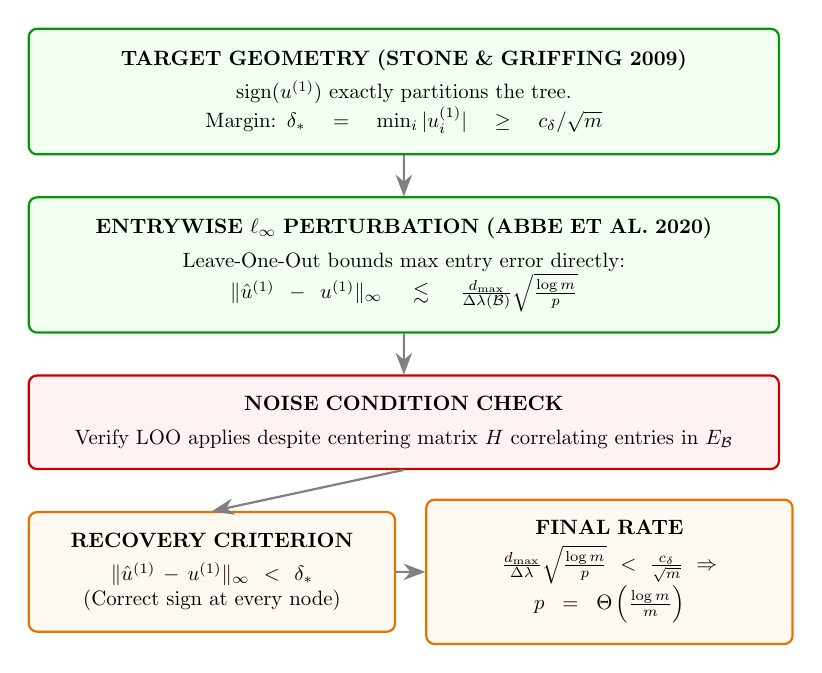
\begin{tikzpicture}[
        scale=0.75, transform shape,
        node distance=0.7cm and 0.5cm,
        box/.style={rectangle, draw, rounded corners=3pt, thick, align=center, inner sep=10pt, text width=12cm},
        boxhalf/.style={rectangle, draw, rounded corners=3pt, thick, align=center, inner sep=10pt, text width=5.5cm},
        cite/.style={draw=green!60!black, fill=green!5},
        prove/.style={draw=red!80!black, fill=red!5},
        deduce/.style={draw=orange!90!black, fill=orange!5},
        arrow/.style={-{Stealth[scale=1.2]}, thick, draw=gray}
    ]
    
    % Nodes
    \node (target) [box, cite] {\textbf{TARGET GEOMETRY (STONE \& GRIFFING 2009)} \\ \vspace{0.15cm} $\text{sign}(u^{(1)})$ exactly partitions the tree. \\ Margin: $\delta_* = \min_i |u_i^{(1)}| \ge c_\delta / \sqrt{m}$};
    
    \node (perturb) [box, cite, below=of target] {\textbf{ENTRYWISE $\ell_\infty$ PERTURBATION (ABBE ET AL. 2020)} \\ \vspace{0.15cm} Leave-One-Out bounds max entry error directly: \\ $\|\hat{u}^{(1)} - u^{(1)}\|_\infty \lesssim \frac{d_{\max}}{\Delta\lambda(\mathcal{B})} \sqrt{\frac{\log m}{p}}$};
    
    \node (noise) [box, prove, below=of perturb] {\textbf{NOISE CONDITION CHECK} \\ \vspace{0.15cm} Verify LOO applies despite centering matrix $H$ correlating entries in $E_{\mathcal{B}}$};
    
    \node (recovery) [boxhalf, deduce, below=of noise, xshift=-3.25cm] {\textbf{RECOVERY CRITERION} \\ \vspace{0.15cm} $\|\hat{u}^{(1)} - u^{(1)}\|_\infty < \delta_*$ \\ (Correct sign at every node)};
    
    \node (rate) [boxhalf, deduce, right=0.5cm of recovery] {\textbf{FINAL RATE} \\ \vspace{0.15cm} $\frac{d_{\max}}{\Delta\lambda} \sqrt{\frac{\log m}{p}} < \frac{c_\delta}{\sqrt{m}} \Rightarrow p = \Theta\left(\frac{\log m}{m}\right)$};
    
    % Arrows
    \draw [arrow] (target) -- (perturb);
    \draw [arrow] (perturb) -- (noise);
    \draw [arrow] (noise.south) -- (recovery.north);
    \draw [arrow] (recovery.east) -- (rate.west);
    
    \end{tikzpicture}
    \caption{The Leave-One-Out (LOO) proof route for single-stage exact recovery.}
    \label{fig:loo_route}
\end{figure}

\subsection{Full Entrywise Proof}

\begin{theorem}[Single-Stage Exact Recovery]
Assume the spectral gap $\Delta\lambda = |\lambda_1(\mathcal{B})| - |\lambda_2(\mathcal{B})|$ is strictly positive. If the sampling rate satisfies
\begin{equation}
p = \Theta\left(\frac{d_{\max}^2}{\Delta\lambda^2 \cdot \delta_*^2} \log m\right)
\end{equation}
then with high probability, $\text{sign}(\hat{u}^{(1)}) = \text{sign}(u^{(1)})$, meaning the raw spectral signs exactly recover the split. For a well-behaved tree where $\Delta\lambda \asymp m$ and $\delta_* \asymp 1/\sqrt{m}$, this yields the standard $p = \Theta(\frac{\log m}{m})$ rate.
\end{theorem}

\begin{proof}
The proof proceeds by bounding the entrywise $\ell_\infty$ error of the eigenvector directly, bypassing the weak $\ell_2$ dimension factor. We deploy the Leave-One-Out (LOO) perturbation framework. For clarity, we restate the relevant consequence of the master theorem from Abbe et al. \cite{abbe2020entrywise}:

\begin{theorem}[Abbe et al. 2020, Theorem 2.1 (Consequence for Symmetric Matrices)]
Let $M$ be a symmetric matrix with eigendecomposition $M = U \Lambda U^\top$, and let $\hat{M} = M + E$ where $E$ is a symmetric noise matrix with independent mean-zero entries (up to symmetry). Let $\hat{U}$ denote the empirical top $r$ eigenvectors. Provided the spectral gap $\Delta\lambda$ is sufficiently large, there exists an orthogonal alignment matrix $W$ such that:
\begin{equation}
\|\hat{U} W - U\|_\infty \lesssim \frac{\|E U\|_\infty}{\Delta\lambda} + \frac{\|E\|_2 \|E\|_{\text{row\_max}}}{\Delta\lambda^2} \|U\|_\infty
\end{equation}
\end{theorem}

In our context, the target signal is the rank-1 leading subspace ($r=1$), so $U$ is the single vector $u^{(1)}$, $W$ is a scalar sign flip (which we resolve by assuming aligned signs), $M$ is the population distance operator $\mathcal{B}$, and $E$ is the centered noise matrix $E_{\mathcal{B}}$. While $\mathcal{B}$ is full rank, the LOO expansion strictly isolates the leading eigenspace gap $\Delta\lambda$, yielding the analogous bound:
\begin{equation}
\|\hat{u}^{(1)} - u^{(1)}\|_\infty \lesssim \frac{\|E_{\mathcal{B}} u^{(1)}\|_\infty}{\Delta\lambda} + \frac{\|E_{\mathcal{B}}\|_2 \|E_{\mathcal{B}}\|_{\text{row\_max}}}{\Delta\lambda^2} \|u^{(1)}\|_\infty
\end{equation}

We now rigorously bound each of the relevant norms for the centered noise matrix $E_{\mathcal{B}} = H E_{\mathcal{D}} H$.

\textbf{1. Bounding the first-order term $\|E_{\mathcal{B}} u^{(1)}\|_\infty$:} \\
Since the population vector is centered ($H u^{(1)} = u^{(1)}$), we have $E_{\mathcal{B}} u^{(1)} = H E_{\mathcal{D}} u^{(1)}$. The $i$-th entry of $E_{\mathcal{D}} u^{(1)}$ is:
\begin{equation}
(E_{\mathcal{D}} u^{(1)})_i = \sum_{j=1}^m (E_{\mathcal{D}})_{ij} u^{(1)}_j
\end{equation}
Because the entries $(E_{\mathcal{D}})_{ij}$ are independent with mean zero, and $u^{(1)}$ is a fixed vector, this is a sum of independent random variables. The variance of the sum is bounded by $\sum_j \frac{d_{\max}^2}{p} (u^{(1)}_j)^2 = \frac{d_{\max}^2}{p}$. The maximum absolute value of a single summand is bounded by $\frac{d_{\max}}{p} \|u^{(1)}\|_\infty$. By Bernstein's inequality, with high probability:
\begin{equation}
\|E_{\mathcal{D}} u^{(1)}\|_\infty \lesssim d_{\max} \sqrt{\frac{\log m}{p}}
\end{equation}
The centering matrix $H$ only subtracts the mean $\frac{1}{m}\mathbf{1}^\top E_{\mathcal{D}} u^{(1)}$, which is an average of these concentrated sums and is therefore of even smaller order. Thus, $\|E_{\mathcal{B}} u^{(1)}\|_\infty \lesssim d_{\max} \sqrt{\frac{\log m}{p}}$.

\textbf{2. Bounding the operator and row norms ($\|E_{\mathcal{B}}\|_2$ and $\|E_{\mathcal{B}}\|_{\text{row\_max}}$):} \\
By standard Matrix Bernstein inequalities \cite{tropp2012}, the operator norm of the independent noise matrix concentrates as $\|E_{\mathcal{D}}\|_2 \lesssim d_{\max} \sqrt{\frac{m}{p}}$. Because $H$ is a projector, $\|E_{\mathcal{B}}\|_2 \le \|E_{\mathcal{D}}\|_2 \lesssim d_{\max} \sqrt{\frac{m}{p}}$. 
Similarly, the row norm $\|e_i^\top E_{\mathcal{B}}\|_2$ is dominated by the Euclidean norm of a row of $E_{\mathcal{D}}$, which is the square root of $m$ independent variables each with variance $d_{\max}^2/p$. By scalar concentration, $\|E_{\mathcal{B}}\|_{\text{row\_max}} \lesssim d_{\max} \sqrt{\frac{m}{p}}$.

\textbf{3. Synthesis and Recovery Criterion:} \\
Substitute these probabilistic bounds into the LOO master equation:
\begin{equation}
\|\hat{u}^{(1)} - u^{(1)}\|_\infty \lesssim \frac{d_{\max}}{\Delta\lambda} \sqrt{\frac{\log m}{p}} + \frac{d_{\max}^2 m}{p \Delta\lambda^2} \|u^{(1)}\|_\infty
\end{equation}
For exact sign recovery, we require this total deviation to be strictly less than the margin $\delta_*$. Assuming standard delocalization where $\|u^{(1)}\|_\infty \asymp 1/\sqrt{m}$ and $\delta_* \asymp 1/\sqrt{m}$, the two terms require:
\begin{equation}
\text{Term 1: } \frac{d_{\max}}{\Delta\lambda} \sqrt{\frac{\log m}{p}} < \frac{c_\delta}{\sqrt{m}} \implies p \gtrsim \frac{d_{\max}^2 m \log m}{\Delta\lambda^2}
\end{equation}
\begin{equation}
\text{Term 2 (H.O.T.): } \frac{d_{\max}^2 m}{p \Delta\lambda^2 \sqrt{m}} < \frac{c_\delta}{\sqrt{m}} \implies p \gtrsim \frac{d_{\max}^2 m}{\Delta\lambda^2}
\end{equation}
Since $\log m > 1$, the first-order term dominates the sample complexity. Thus, $p = \Theta\left( \frac{d_{\max}^2 m \log m}{\Delta\lambda^2} \right)$ is sufficient for exact sign recovery. 
\end{proof}

\subsection{Open Question: How Do $\Delta\lambda$ and $\delta_*$ Depend on the Tree?}

The rate above is written in terms of two numbers, and both are fixed as soon as the tree
is fixed --- no sampling enters either one:
\begin{itemize}
\item the gap $\Delta\lambda = |\lambda_1(\mathcal{B})| - |\lambda_2(\mathcal{B})|$, which
says how far the leading direction of $\mathcal{B}$ stands out from the next one;
\item the smallest entry $\delta_* = \min_i |u^{(1)}_i|$, which says how close the closest
leaf comes to sitting on the fence between the two sides.
\end{itemize}
We put $\Delta\lambda \asymp m$ and $\delta_* \asymp 1/\sqrt{m}$ into the general rate to
get $p \gtrsim \log m / m$. What is open is how to read those two numbers off a tree:

\begin{quote}
Given a weighted tree $T$ with $m$ leaves, how small can $\Delta\lambda$ and $\delta_*$
be, in terms of the shape of $T$ and the lengths of its branches?
\end{quote}

The two travel together. The vector $u^{(1)}$ is the direction that maximises the Rayleigh
quotient of $\mathcal{B}$, so a tree that leaves little room between the first and second
directions is also a tree whose leading vector comes close to zero somewhere. A useful
reference point: if $u^{(1)}$ were exactly two-valued, one value on each side of a split
that puts a fraction $\alpha \le 1/2$ of the leaves on the smaller side, then centering and
unit length fix its entries, and the smaller of the two is
\begin{equation}
\label{eq:two-block-margin}
\delta_* = \frac{1}{\sqrt{m}}\sqrt{\frac{\alpha}{1-\alpha}} .
\end{equation}
So the margin is set by how lopsided the split is, and $\alpha$ is something the tree model
decides. \Cref{tab:tree-kinds} collects what each kind of tree does to the two numbers.

\begin{table}[H]
\centering
\begin{tabular}{@{}p{2.9cm}p{3.1cm}p{2.7cm}p{5.2cm}@{}}
\toprule
Tree & $\delta_* \approx$ & $\Delta\lambda \approx$ & Note \\
\midrule
Balanced binary
  & $1/\sqrt{m}$
  & order $m$
  & Symmetry fixes the vector: it is close to two-valued with $\alpha = 1/2$, so every
    entry has about the same size. \\[4pt]
Kingman coalescent
  & $\sqrt{\alpha/(1-\alpha)}\,/\sqrt{m}$
  & a constant fraction of $|\lambda_1|$
  & Theory: the topology is Yule, whose root split is uniform in size
    \cite{steel2001yule,aldous2001stochastic}, so the smaller side $\alpha$ is uniform on
    $\{1/m,\dots,1/2\}$; it is typically of order one and
    $\delta_*$ of order $1/\sqrt{m}$, with a tail down to $1/m$ when the split peels off a
    single leaf. The last coalescence lasts $\mathrm{Exp}(1)$ against a tree height of mean
    $2(1-1/m)$ \cite{kingman1982coalescent,wakeley2009coalescent}, so the deepest split
    stands clear of the next one by a fixed proportion. Both are borne out in
    \Cref{fig:app-eig,fig:app-vec}. \\[4pt]
Pure birth (Yule branch lengths)
  & $0.024/\sqrt{m}$
  & $0.38\,|\lambda_1|$
  & Same topology law as the row above, so the same $\alpha$; what changes is where the
    branch lengths sit. Medians over $200$ trees at $m=1000$, against $0.36/\sqrt{m}$ and
    $0.60\,|\lambda_1|$ for the coalescent; see \Cref{fig:app-eig,fig:app-vec}. \\[4pt]
Caterpillar, very uneven branch lengths (extreme)
  & well below $1/\sqrt{m}$
  & well below $m$
  & The vector puts most of its weight on a handful of leaves and the rest of the entries
    are tiny, which is $\alpha \to 1/m$ in \eqref{eq:two-block-margin}. How far below is
    the open part. \\
\bottomrule
\end{tabular}
\caption{What each kind of tree does to the two numbers the rate is written in.}
\label{tab:tree-kinds}
\end{table}

So one half of the assumption in \Cref{sec:target} is comfortable and the other half is
where the work is. The bound $\|u^{(1)}\|_\infty \le C_\delta/\sqrt{m}$ holds on both
random models with a small constant. The margin $\delta_* \ge c_\delta/\sqrt{m}$ is the
half that a tree can push down, and since $p$ scales as $1/\delta_*^2$, a margin ten times
smaller asks for a hundred times more of the matrix. The general form
$p \gtrsim d_{\max}^2 \log m / (\Delta\lambda^2 \delta_*^2)$ covers all three rows; what
each row needs is the right pair of numbers to put into it.

\appendix

\section{The two operators on simulated trees}
\label{app:operators}

% [Reviewer Note: this appendix supplies the empirical picture behind the two quantities
% the open question in Section 1.4 is stated in --- the gap Delta-lambda and the margin
% delta_*. Assets are produced by analysis/supporting/eta_by_operator.ipynb (final cell)
% and live in figures/dr2_*.png.]

The quantities the recovery rate is stated in, $\Delta\lambda$ and $\delta_*$, are
properties of the population operator, so they can be read off simulated trees exactly.
The figures below do that on Jukes--Cantor sequences of length $L=10^4$ over trees with
$m=1000$ leaves: one tree for the anatomy of a single split
(\Cref{fig:app-tree,fig:app-mat}), and pools of $200$ Kingman and $200$ birth--death
trees for the distributions (\Cref{fig:app-eig,fig:app-vec}). Throughout, $\mathcal{B}$
is compared against the graph Laplacian $L(S)=\mathrm{Deg}(S)-S$ of the similarity matrix
$S=e^{-\mathcal{D}}$, whose Fiedler vector is the alternative classifier.

\begin{figure}[H]
    \centering
    \begin{subfigure}[t]{0.46\textwidth}
        \captionsetup{singlelinecheck=false, justification=raggedright, skip=1pt}
        \subcaption{Fiedler vector of $L(S)$}
        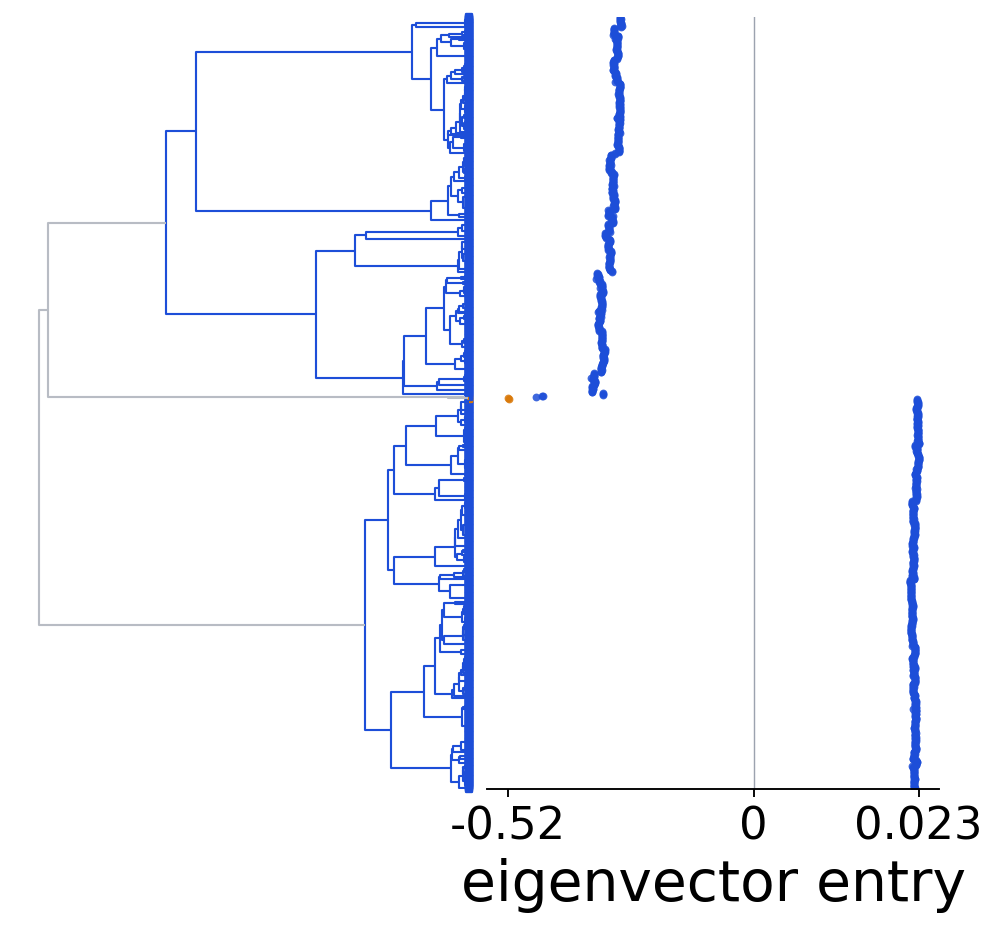
\includegraphics[width=\textwidth]{figures/dr2_tree_vec_S.png}
        \label{fig:app-tree-a}
    \end{subfigure}
    \hfill
    \begin{subfigure}[t]{0.46\textwidth}
        \captionsetup{singlelinecheck=false, justification=raggedright, skip=1pt}
        \subcaption{$u^{(1)}$ of $\mathcal{B}=H\mathcal{D}H$}
        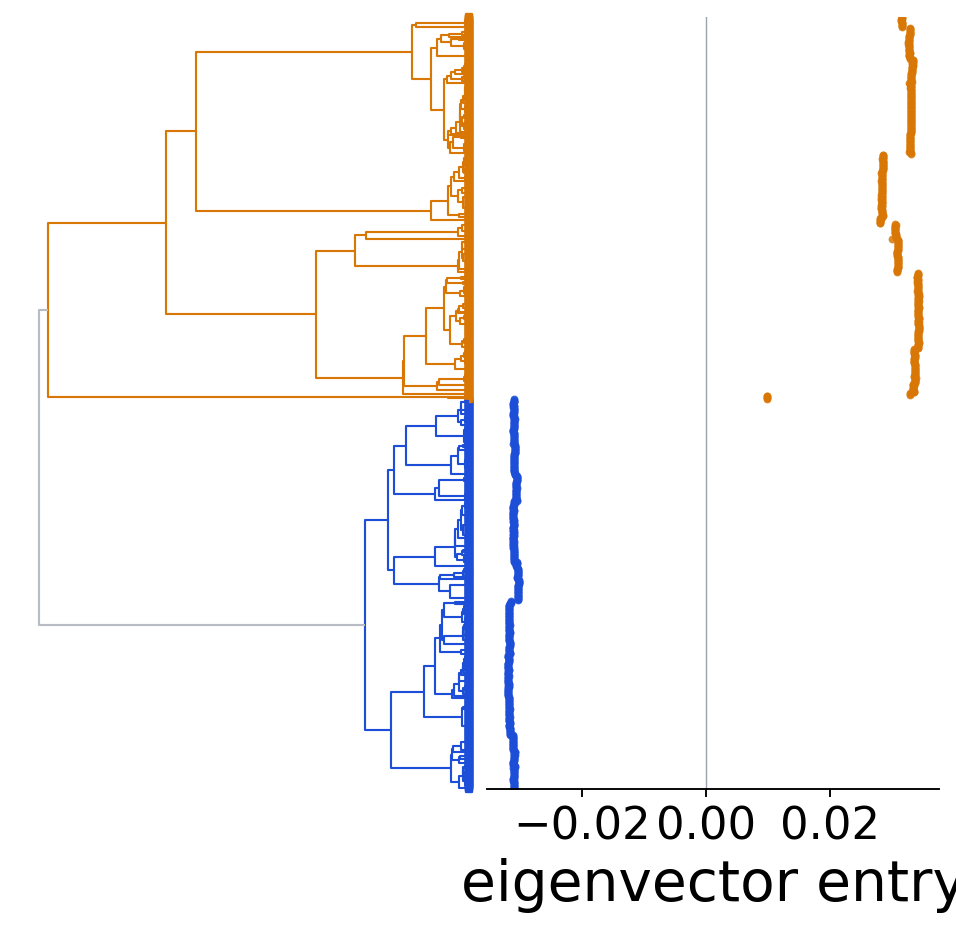
\includegraphics[width=\textwidth]{figures/dr2_tree_vec_B.png}
        \label{fig:app-tree-b}
    \end{subfigure}
    \caption{One Kingman tree, drawn twice, each copy cut by its own vector: blue and
    orange are the two sides of that cut, grey a clade straddling it, and the scatter
    holds the vector entries in the same leaf order. The tree shown is the one in the
    pool where the two cuts differ most: $u^{(1)}$ splits it $505/495$, the Fiedler
    vector $998/2$.}
    \label{fig:app-tree}
\end{figure}

The two vectors are read off two different matrices built from the same alignment, shown next in the same leaf order.

\begin{figure}[H]
    \centering
    \begin{subfigure}[t]{0.24\textwidth}
        \captionsetup{singlelinecheck=false, justification=raggedright, skip=1pt}
        \subcaption{$S=e^{-\mathcal{D}}$}
        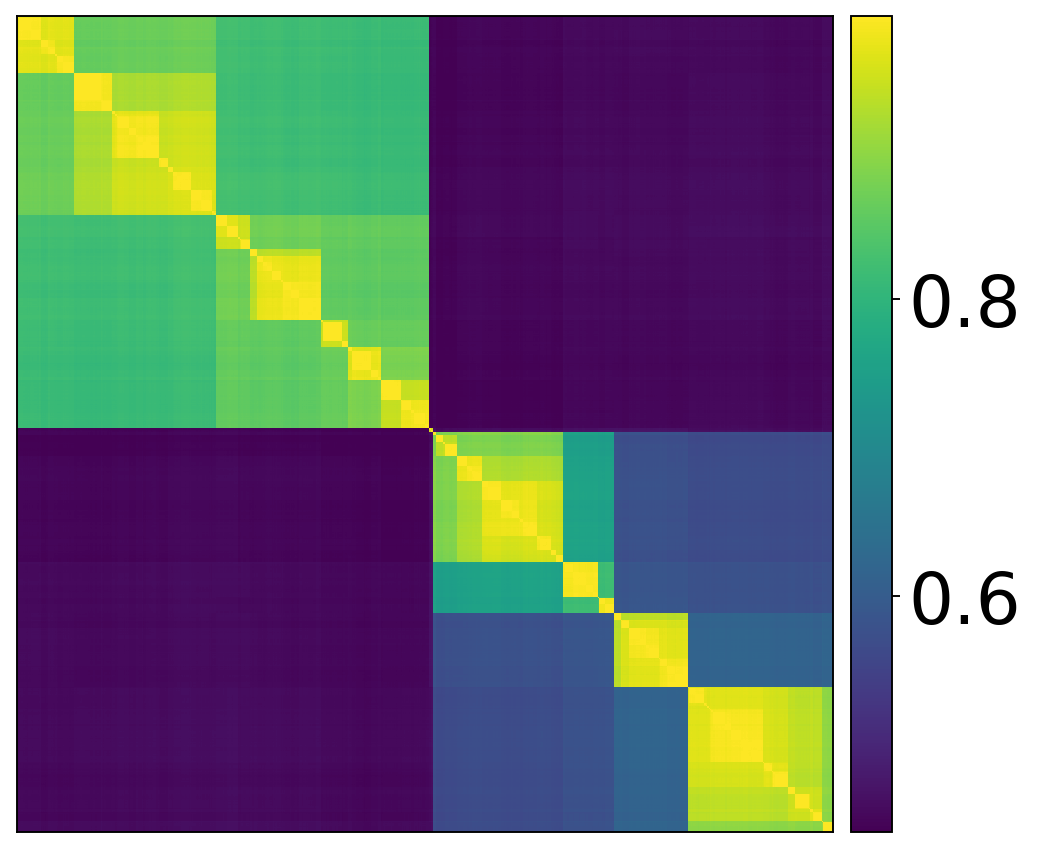
\includegraphics[width=\textwidth]{figures/dr2_mat_S.png}
    \end{subfigure}
    \hfill
    \begin{subfigure}[t]{0.24\textwidth}
        \captionsetup{singlelinecheck=false, justification=raggedright, skip=1pt}
        \subcaption{$L(S)=\mathrm{Deg}(S)-S$}
        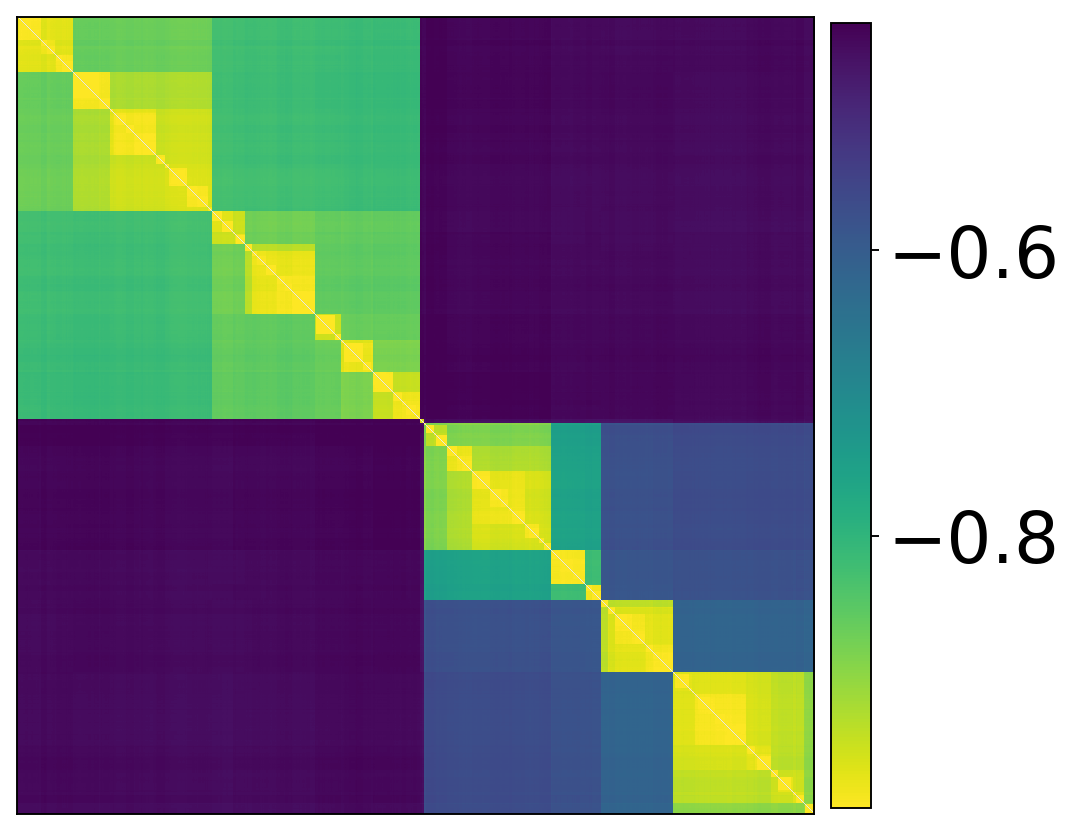
\includegraphics[width=\textwidth]{figures/dr2_mat_L.png}
    \end{subfigure}
    \hfill
    \begin{subfigure}[t]{0.24\textwidth}
        \captionsetup{singlelinecheck=false, justification=raggedright, skip=1pt}
        \subcaption{$\mathcal{D}=-\log S$}
        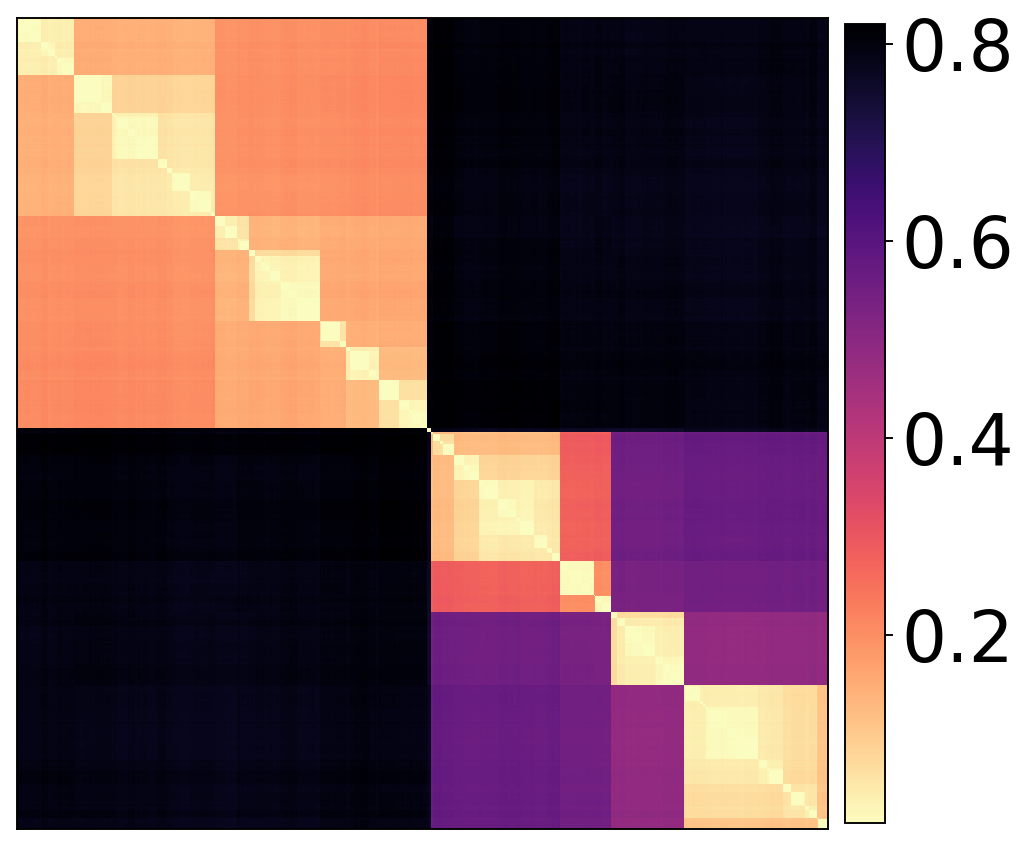
\includegraphics[width=\textwidth]{figures/dr2_mat_D.png}
    \end{subfigure}
    \hfill
    \begin{subfigure}[t]{0.24\textwidth}
        \captionsetup{singlelinecheck=false, justification=raggedright, skip=1pt}
        \subcaption{$\mathcal{B}=H\mathcal{D}H$}
        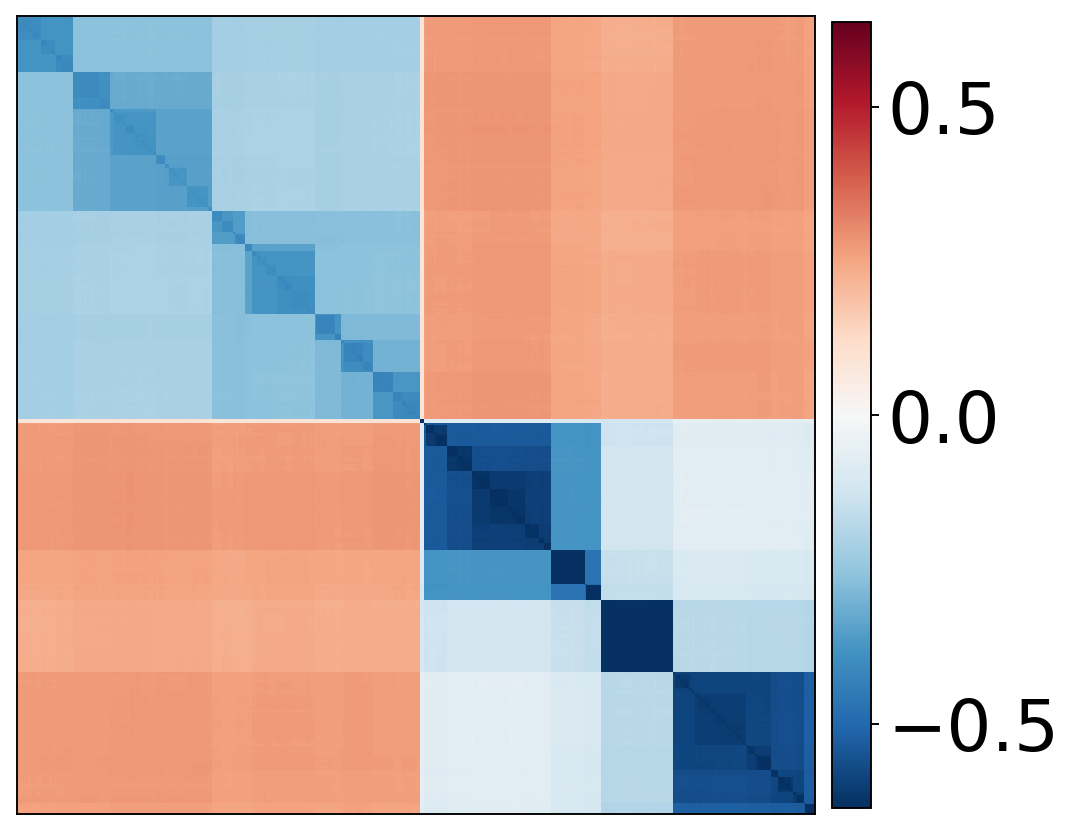
\includegraphics[width=\textwidth]{figures/dr2_mat_B.png}
    \end{subfigure}
    \caption{The four matrices on the tree of \Cref{fig:app-tree}, leaves ordered so that
    a clade is a contiguous block. Each panel carries its own colour scale: the diagonal
    of $L(S)$ is the degree, three orders above its off-diagonal, and is masked in grey;
    $\mathcal{B}$ is signed and shown diverging about zero.}
    \label{fig:app-mat}
\end{figure}

Across the pools, the quantity that governs the rate is the separation between the first two eigenvalues.

\begin{figure}[H]
    \centering
    \begin{subfigure}[t]{0.42\textwidth}
        \captionsetup{singlelinecheck=false, justification=raggedright, skip=1pt}
        \subcaption{Kingman, $L(S)$}
        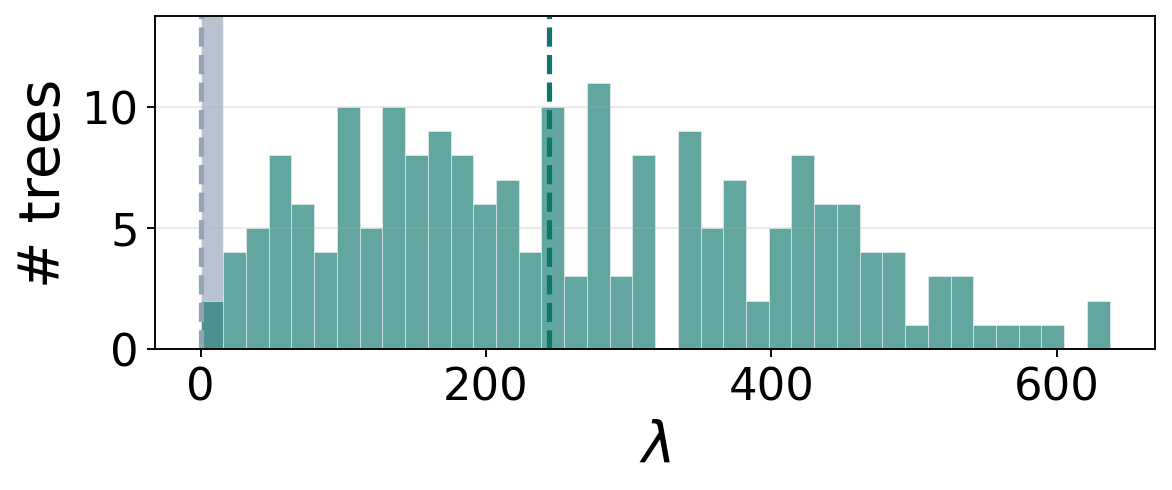
\includegraphics[width=\textwidth]{figures/dr2_eig_kingman_L.png}
    \end{subfigure}
    \hfill
    \begin{subfigure}[t]{0.42\textwidth}
        \captionsetup{singlelinecheck=false, justification=raggedright, skip=1pt}
        \subcaption{Kingman, $\mathcal{B}$}
        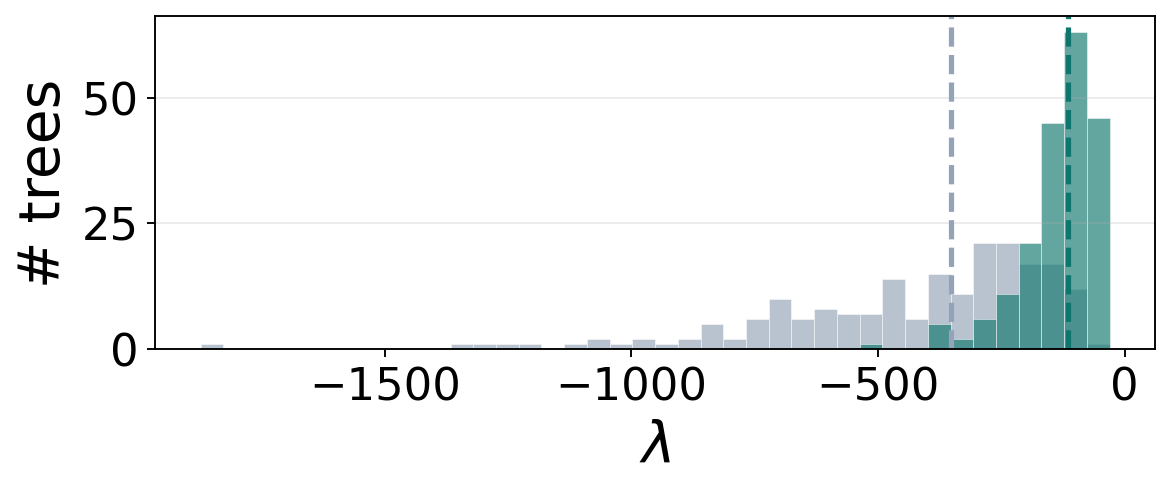
\includegraphics[width=\textwidth]{figures/dr2_eig_kingman_B.png}
    \end{subfigure}

    \begin{subfigure}[t]{0.42\textwidth}
        \captionsetup{singlelinecheck=false, justification=raggedright, skip=1pt}
        \subcaption{birth--death, $L(S)$}
        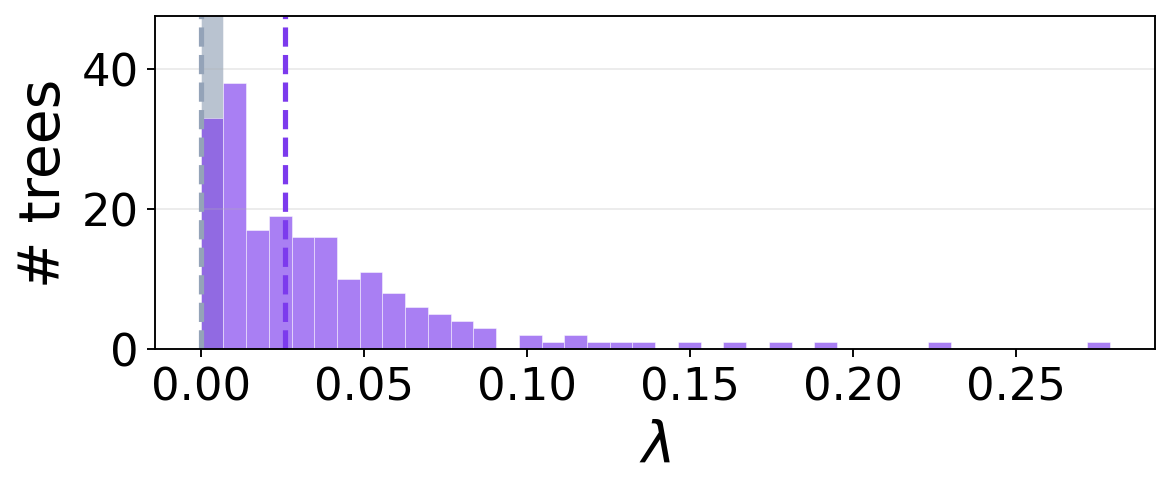
\includegraphics[width=\textwidth]{figures/dr2_eig_bd_L.png}
    \end{subfigure}
    \hfill
    \begin{subfigure}[t]{0.42\textwidth}
        \captionsetup{singlelinecheck=false, justification=raggedright, skip=1pt}
        \subcaption{birth--death, $\mathcal{B}$}
        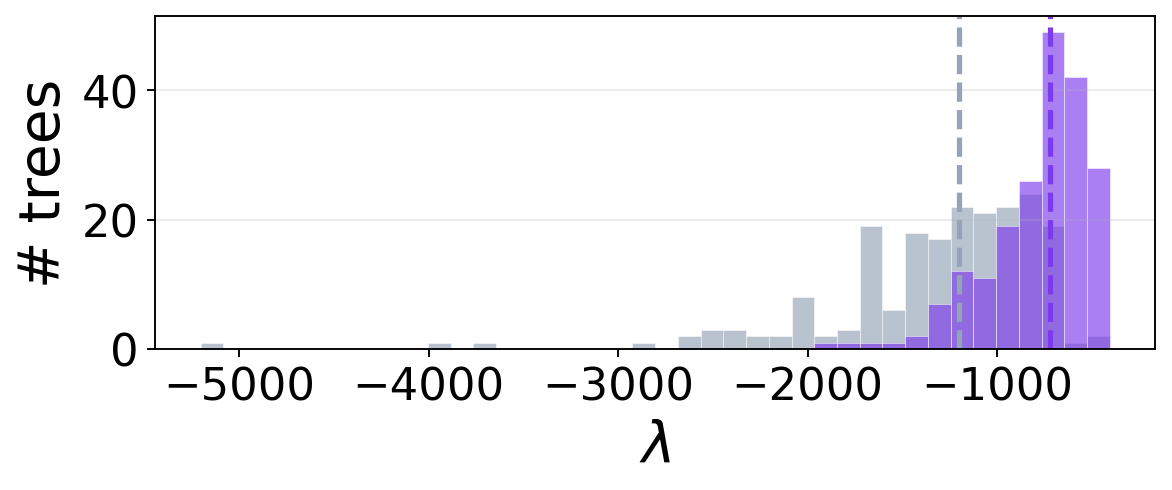
\includegraphics[width=\textwidth]{figures/dr2_eig_bd_B.png}
    \end{subfigure}
    \caption{Distribution over $200$ trees per model of the two leading eigenvalues of
    each operator: grey $\lambda_1$, coloured $\lambda_2$, dashed lines at the medians.
    For $L(S)$ the eigenvalues are ascending and $\lambda_1\equiv0$, so its bar is
    clipped; for $\mathcal{B}$ they are the two largest in magnitude, both negative.
    The relative gap $(|\lambda_1|-|\lambda_2|)/|\lambda_1|$ of $\mathcal{B}$ has median
    $0.60$ on Kingman trees and $0.38$ on birth--death trees, against $0.20$ and $0.25$
    for the corresponding Fiedler gap $(\lambda_3-\lambda_2)/\lambda_3$.}
    \label{fig:app-eig}
\end{figure}

The margin $\delta_*$ is a property of the entries themselves, pooled below over the same trees.

\begin{figure}[H]
    \centering
    \begin{subfigure}[t]{0.42\textwidth}
        \captionsetup{singlelinecheck=false, justification=raggedright, skip=1pt}
        \subcaption{Kingman, Fiedler of $L(S)$}
        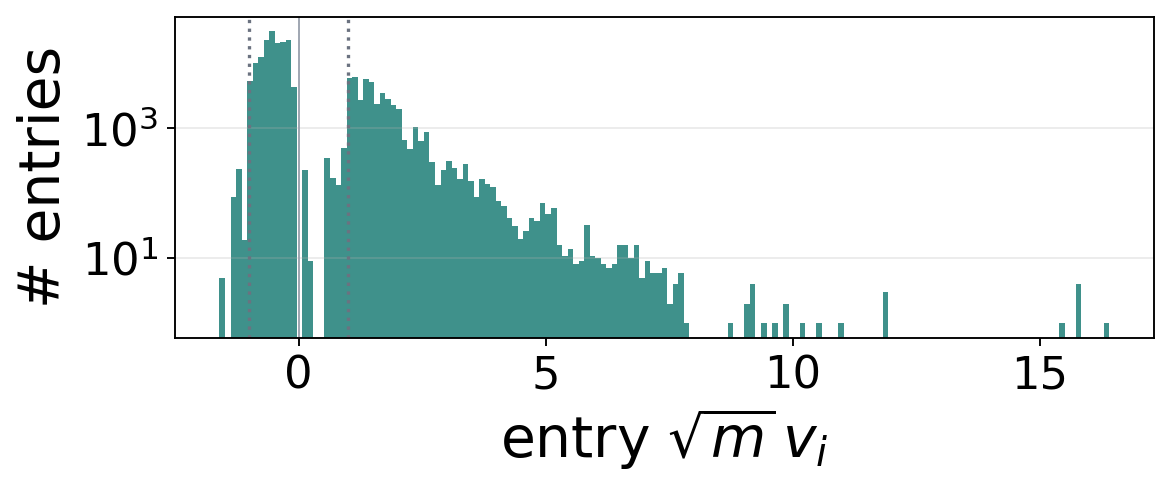
\includegraphics[width=\textwidth]{figures/dr2_vec_kingman_L.png}
    \end{subfigure}
    \hfill
    \begin{subfigure}[t]{0.42\textwidth}
        \captionsetup{singlelinecheck=false, justification=raggedright, skip=1pt}
        \subcaption{Kingman, $u^{(1)}$}
        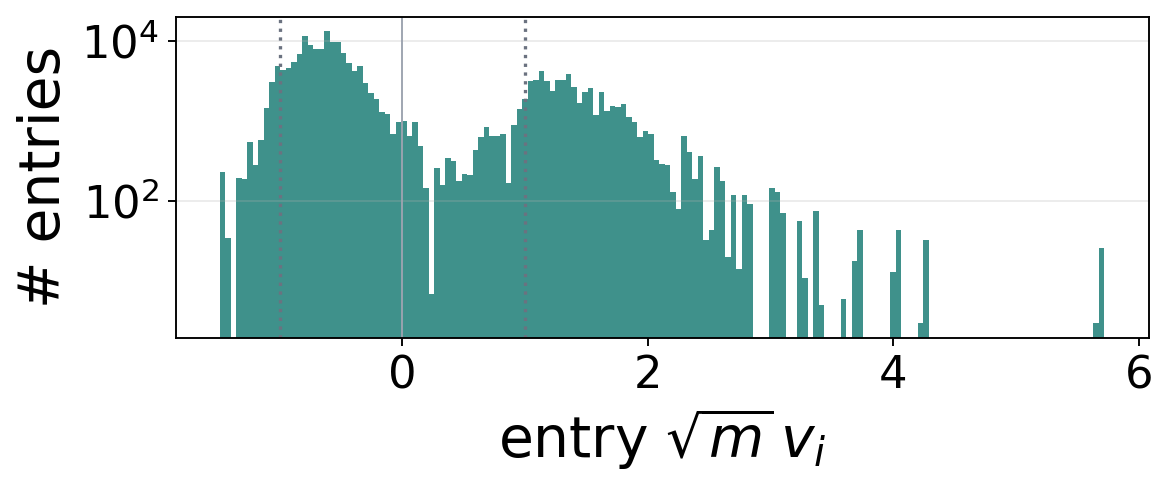
\includegraphics[width=\textwidth]{figures/dr2_vec_kingman_B.png}
    \end{subfigure}

    \begin{subfigure}[t]{0.42\textwidth}
        \captionsetup{singlelinecheck=false, justification=raggedright, skip=1pt}
        \subcaption{birth--death, Fiedler of $L(S)$}
        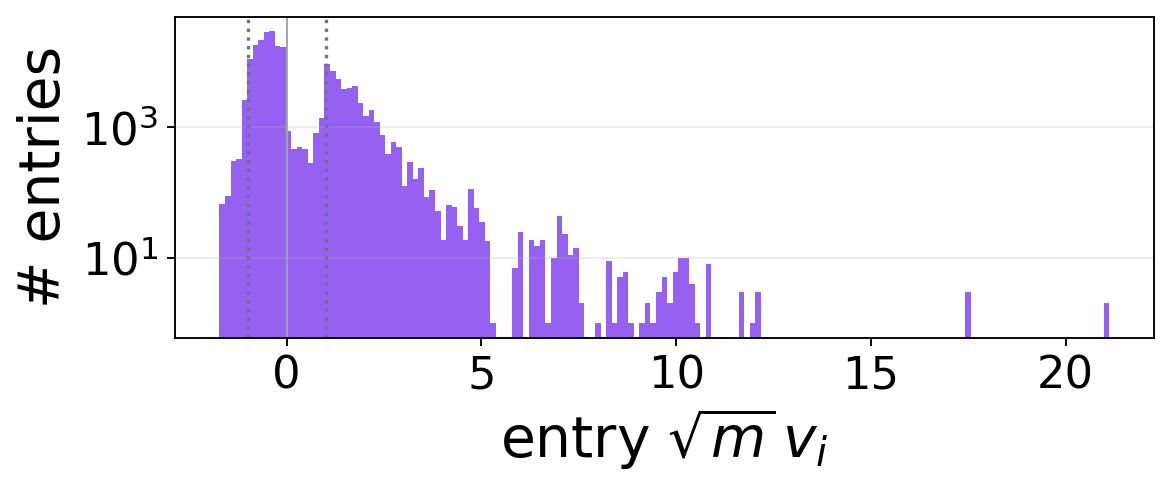
\includegraphics[width=\textwidth]{figures/dr2_vec_bd_L.png}
    \end{subfigure}
    \hfill
    \begin{subfigure}[t]{0.42\textwidth}
        \captionsetup{singlelinecheck=false, justification=raggedright, skip=1pt}
        \subcaption{birth--death, $u^{(1)}$}
        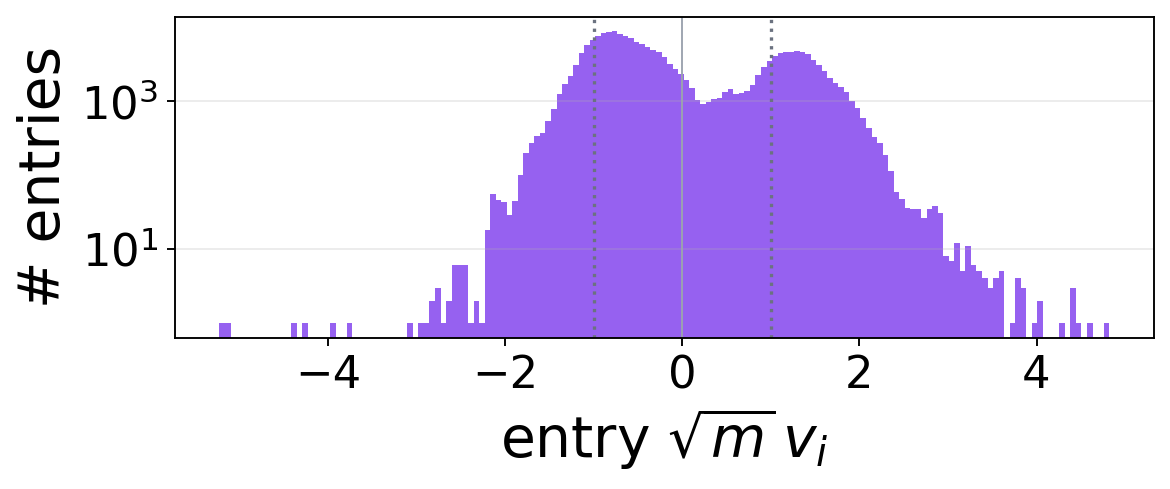
\includegraphics[width=\textwidth]{figures/dr2_vec_bd_B.png}
    \end{subfigure}
    \caption{Entries of the classifying vector, pooled over the same $200$ trees per
    model, each vector normalised to $\|v\|=1$, scaled by $\sqrt{m}$ and oriented with
    the minority side positive; counts are logarithmic and the dotted lines mark
    $\pm1$, the value a perfectly delocalised vector takes. The entries of $u^{(1)}$
    cluster at $\pm1$ with a largest entry of $5.7$ against $\sqrt{m}=31.6$, which is
    the delocalisation $\|u^{(1)}\|_\infty \asymp 1/\sqrt{m}$ assumed in
    Section~\ref{sec:target}; the Fiedler vector reaches $16.4$ on Kingman trees and $21.1$ on birth--death trees.}
    \label{fig:app-vec}
\end{figure}

\newpage
\bibliographystyle{plain}
\bibliography{bibi}

\end{document}